\documentclass[10pt,twocolumn,letterpaper]{article}

\usepackage{iccp}
\usepackage{times}
\usepackage{amsmath}
\usepackage{amssymb}
\usepackage{url}
\usepackage{graphicx}
\DeclareMathOperator*{\argmin}{\arg\!\min}
% for rapid builds, with bounding boxes instead of images add the [draft] option to graphicx
% \usepackage[draft]{graphicx}

\iccpfinalcopy % *** Uncomment this line for the final submission

\def\iccpPaperID{****} % *** Enter the ICCP Paper ID here
\def\httilde{\mbox{\tt\raisebox{-.5ex}{\symbol{126}}}}

% Pages are numbered in submission mode, and unnumbered in camera-ready
\ificcpfinal\pagestyle{empty}\fi
\begin{document}

%%%%%%%%% TITLE
\title{Comparison of Sparsity in Different Basis for Lightfields}

\author{Philip K. Lee\\
Stanford University\\
Electrical Engineering Department\\
{\tt\small pkl.lee@stanford.edu}
\and
Anqi R. Ji\\
Stanford University\\
Electrical Engineering Department\\
{\small\url{anqi@stanford.edu}}
}

\maketitle
\thispagestyle{empty}

%%%%%%%%% ABSTRACT
\begin{abstract}

\end{abstract}

\section{Introduction}

Different methods of capturing the 4D light field exist, which balance a tradeoff between spatial and angular resolution, and require additional hardware and capture times. These methods include a microlens array mounted in front of the camera sensor \cite{NgLF}, which comes at the cost of spatial resolution, and camera arrays \cite{LFArray} or cameras mounted on a mechanical gantry \cite{LFRendering}. Sparse reconstruction of the light field is desirable as it helps to alleviate some of these tradeoffs. Priors that exploit the sparsity of the light field in some dimension allow the entire light field to be reconstructed from a limited number of samples. For example, the light field can be considered to be sparse in the angular domain due to the light field being the same scene acquired from slightly different perspective. 

Multiple methods have been applied to reconstruct the light field from a sparse set of samples. 

In \cite{DimGapLFPrior}, a Lambertian scene is assumed and a 3D Gaussian prior is applied to the scene. This prior comes from the observation that the 4D Fourier transform of the 4D ray space contains a 3D subset of entries whose energy is significantly higher than zero. Under this prior, the light field can be recovered using spatial deconvolutions with a depth invariant Point Spread Function. Though this method is easy to compute, it creates artifacts in non-Lambertian scenes.

A second approach applied in \cite{LFDict} recovers the light field using a randomly coded attenuation mask and dictionaries derived from training data acquired from other light field images. The dictionaries are then applied to solve the ill-posed problem of recovering the entire light field from a random linear combination of light field samples provided by the coded mask.

Compressive sensing \cite{IntroCS}\cite{CompressiveSensingMega} is another approach to reconstruction of the light field using sparse samples. By applying a randomly-coded aperture mask to the lens, the authors of \cite{SparsityInCFD} were able to reconstruct the light field with a superior angular resolution and SNR compared to sequentially opening and blocking small regions of the aperture. The light field is recovered using a Bayesian reconstruction model with Total Variation and Gaussian priors. A Majorize-Minimization optimization was used to recover the light field.

In order to achieve the best reconstruction using compressive sensing, it is desirable to perform the reconstruction in the basis in which the original signal is most sparse, as a higher percentage of the signal's energy will be concentrated in fewer coefficients of the sparse basis \cite{CompressiveSensingMega}. Therefore it is advantageous to determine in what basis the angular lightfield is most sparse. This was explored in part in \cite{mainP1}, but only the basis that yielded the best reconstruction for each compression was shown. The goal of our work is to experimentally determine the basis in which lightfields are most sparse by performing sparse reconstructions of the lightfield for different compression factors. We use images captured from a Lytro Illum camera available from the Stanford Lytro Light Field Archive \footnote{Available: \url{lightfields.stanford.edu}} to simulate measurements and determine the reconstruction error for different basis.

\section{Background}

In the background, we present the basic mathematics for compressed sensing and recovery using the total variance prior.

\subsection{Compressed Sensing}

In this section we present the formulation of the compressed sensing framework \cite{CSPaper} for the general case and for lightfields. A signal $x \in \mathbb{R}^N$ which is $K$-sparse in some basis $\Phi \in \mathbb{R}^{N\times N}$, i.e.,

\[ x = \Phi \theta, \quad ||\theta||_0 = K, \quad K \ll N\]

can be recovered using a smaller vector $y \in \mathbb{R}^M, M < K < N$, where $y$ is a vector consisting of linear combinations of $x$. In matrix notation, $y$ can be expressed as 

\[ y = \Psi x, \quad \Psi \in \mathbb{R}^{M \times N}\]

$\Psi$ is known as the sensing matrix. There are many ways to generate $\Psi$ that would allow for sparse recovery using a limited number of measurements. One such method is to use a $\Psi$ whose elements are drawn from a Gaussian or Bernoulli distribution, but this choice is determined by the physical limitations of the problem \cite{Rauhut11}. The vector $x$ can be recovered as $\hat{x}$ if $M$ is large enough ($M \sim K\log(N/K)$) by finding the optimum solution for 

\[ \hat{\theta} = \argmin_\theta ||\theta||_0 \quad s.t. \quad \Psi\Phi\theta = y\]

and recovering $\hat{x}$ using

\[ \hat{x} = \Phi \hat{\theta}\]

Intuitively, this optimization seeks to concentrate the energy of the reconstructed signal in as few coefficients as possible in the sparse basis, while also ensuring that applying the sensing matrix to the reconstructed signal is close to the measurements. However, $l_0$ optimization is NP-hard, so instead we resort to the $l_1$ norm which approximates the $l_0$ norm

\[ \hat{\theta} = \argmin_\theta ||\theta||_1 \quad s.t. \quad \Psi\Phi\theta = y\]

This problem is known as Basis Pursuit (BP) \cite{BasisPursuit1}. For the general case with added noise in the measurements, the problem becomes

\[ \hat{\theta} = \argmin_\theta ||\theta||_1 \quad s.t. \quad ||\Psi\Phi\theta - y||_2 < \sigma\]


where $\sigma$ is a bound for the noise in the measurements. This is the Basis Pursuit Denoise (BPDN) problem. In our work, we only consider Basis Pursuit.

\subsection{Compressed Sensing for Lightfields}

In the background, we considered the reconstruction of signals in 1 dimension. However, a lightfield exists in 4 dimensions: the spatial dimensions $x, y$ and the angular dimensions $u, v$. In this section, we will recast the problem in terms of the dimensions for a 4D lightfield. Note that the dimensions for the matrix multiplications may not align, but this section is included to clarify the reconstruction for 4D lightfields.

Consider a lightfield $L \in \mathbb{R}^{w \times h \times n \times n}$, where $w$ and $h$ are respectively the width and height of each angular image. For simplicity, we assume that the number of angular lightfield views $n$ is equal in each dimension. We wish to recover $L$ using only linear combinations of $L$.

Our sensing matrix $\Psi$ operates on the angular images, therefore $\Psi$ is of size $\mathbb{R}^{M \times n \times n}$ where $M$ is the number of measurements. Our measured data is therefore

\[Y = \Psi L, \quad Y \in \mathbb{R}^{w \times h \times M}\]

The orthogonal basis $\Phi$ operates in the angular domain, so $\Phi \in \mathbb{R}^{n \times n}$. The BP problem becomes

\[ \hat{\theta} = \argmin_\theta ||\theta||_1 \quad s.t. \quad \Psi\Phi\theta = Y\]
\[ \hat{\theta}, \theta \in \mathbb{R}^{w \times h \times n \times n}\]

and the lightfield is recovered using

\[ \hat{L} = \Phi \hat{\theta}\]

To solve the BP problem, it is convenient to let the matrix $A = \Psi\Phi$. We can now define the adjoint operator as $A' = \Phi'\Psi'$ where the $'$ denotes the transpose. Since $\Phi$ is orthonormal, $\Phi'\Phi = I$, so $\Phi'$ is the inverse of the basis operator. 

\subsection{Total Variation Prior}

Unlike compressed sensing which assumes sparsity in some orthogonal basis, Total Variation (TV) assumes sparsity in the gradients of the image. This is achieved by minimizing the following cost function

\[ \hat{x} = \argmin_x ||Ax - b||^2_2 + \lambda ||D x||_1 \]

Where $D$ is the gradient operator and $\lambda$ is a parameter that can be chosen. A larger choice of $\lambda$ will reduce the amount of edges in the image. $A$ is similar to the sensing matrix presented above and constitutes the masks used to generate the measurements $b$.

\section{Methods}


24 images were chosen at random from the Stanford Lytro Light Field Archive \footnote{Available: \url{lightfields.stanford.edu}}. Images captured using the Lytro Illum camera have a raw resolution of $7574 \times 5264$ pixels, and has $14 \times 14$ angular views over the RGB colour channels. Each angular view has a resolution of $541 \times 376$. Our simulations reduced the resolution of each angular view by a factor of $6$ using bilinear interpolation in order to reduce reconstruction time. Only the center $10 \times 10$ angular views of each image were considered for the simulation as the microlens array in the Lytro camera causes pixels at the edge to be obscured.

The sensing matrix was created for multiple compression factors by drawing the elements from a Uniform distribution \cite{Rauhut11}. The uniform distribution is a good approximation for random attenuation masks.

The sparse reconstruction was solved using SPGL1\footnote{\url{http://www.cs.ubc.ca/~mpf/spgl1/}} \cite{BasisPursuit1}\cite{BasisPursuit2}. We used the Basis Pursuit solver for the recovery. $1500$ iterations was sufficient to converge on the solution.

The reconstruction was performed using the following orthonormal basis: DCT, Fourier, and Haar Wavelets, and by minimizing the TV cost function.


Reconstructions were performed in parallel for different compression ratios and basis using the Barley machines on the Stanford Farmshare cluster. Each Barley machine is equipped with an AMD Magny Cours (24 cores each) and is shared across multiple users. The approximate time for reconstructing a $90 \times 63 \times 10 \times 10$ lightfield using a particular reconstruction method is shown in Table 1.

\begin{table}
  \begin{center}
  \begin{tabular}{|l|c|}
  \hline
  Basis & Reconstruction Time (hours)\\
  \hline\hline
  Fourier & 12.3 \\
  DCT & 12.4 \\
  Haar & 16.8\\
  TV Prior & 5.1\\ 
  \hline
  \end{tabular}
  \end{center}
  \caption{Reconstruction times for a single lightfield image using the Barley machines.}
\end{table}


We define the SNR as the energy in the original signal divided by the mean squared error of the reconstruction across all colour channels. 

\[SNR = 20 \log_{10}{\frac{||x||_2}{||x_r - x||_2}}\] where $x$ is the original lightfield image, and $x_r$ is the reconstructed lightfield image and $|| \cdot ||_2$ is the $l2$ norm.

We define the compression ratio as the number of measuremnts $M$ divided by the number of angular views \[ \eta = \frac{M}{N} = \frac{M}{n \times n}\]

\section{Results}

SNR graphs for different compression basis
Select images

\begin{figure}[t]
\begin{center}
\fbox{\rule{0pt}{2in} \rule{0.9\linewidth}{0pt}}
 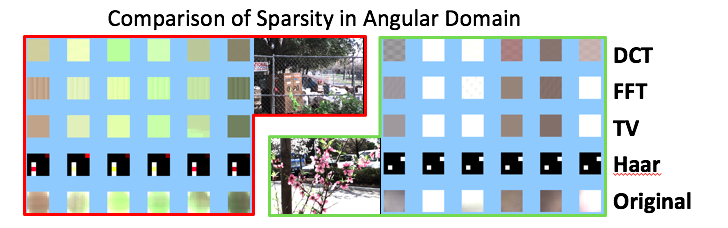
\includegraphics[width=0.8\linewidth]{img/patches.png}
\end{center}
   \caption{Example of caption.  It is set in Roman so that mathematics
   (always set in Roman: $B \sin A = A \sin B$) may be included without an
   ugly clash.}
\end{figure}


\begin{figure}[t]
\begin{center}
\fbox{\rule{0pt}{2in} \rule{0.9\linewidth}{0pt}}
 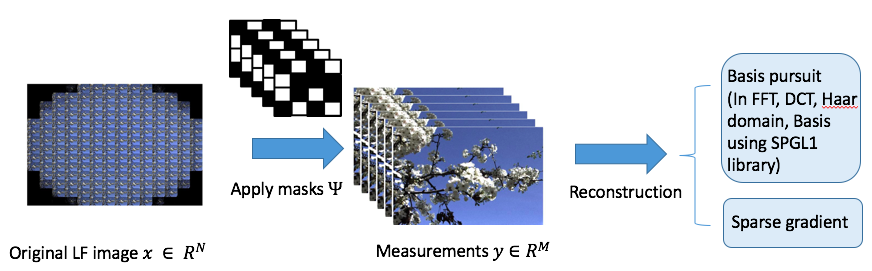
\includegraphics[width=0.8\linewidth]{img/cs_framework.png}
\end{center}
   \caption{Example of caption.  It is set in Roman so that mathematics
   (always set in Roman: $B \sin A = A \sin B$) may be included without an
   ugly clash.}
\end{figure}

\section{Discussion}

\section{Conclusion}



{\small
\bibliographystyle{ieee}
\bibliography{egbib}
}

\end{document}
